% Initial System Characterization

\documentclass[9pt]{article} % use larger type; default would be 10pt

\usepackage[utf8]{inputenc} % set input encoding (not needed with XeLaTeX)
\usepackage{amsmath}
\usepackage{graphicx}
\usepackage{multicol}
\setlength{\columnsep}{0.5cm}
\usepackage[backend=biber]{biblatex}
\usepackage[margin=1.0in]{geometry}
\usepackage{siunitx}
\addbibresource{references.bib}

% For two figures side-by-side
\usepackage{mwe}
\usepackage[font=small]{caption}


\numberwithin{equation}{section} % number within sections
% \usepackage[parfill]{parskip} % new line without indent

%%% Examples of Article customizations
% These packages are optional, depending whether you want the features they provide.
% See the LaTeX Companion or other references for full information.

%%% PAGE DIMENSIONS
\usepackage{changepage} % to adjust margins for a single paragraph
\usepackage{geometry} % to change the page dimensions
\geometry{a4paper} % or letterpaper (US) or a5paper or....
% \geometry{margin=2in} % for example, change the margins to 2 inches all round
% \geometry{landscape} % set up the page for landscape
%   read geometry.pdf for detailed page layout information

\usepackage{graphicx} % support the \includegraphics command and options

% \usepackage[parfill]{parskip} % Activate to begin paragraphs with an empty line rather than an indent

%%% PACKAGES
\usepackage{booktabs} % for much better looking tables
\usepackage{array} % for better arrays (eg matrices) in maths
\usepackage{paralist} % very flexible & customisable lists (eg. enumerate/itemize, etc.)
\usepackage{verbatim} % adds environment for commenting out blocks of text & for better verbatim
\usepackage{subfig} % make it possible to include more than one captioned figure/table in a single float
% These packages are all incorporated in the memoir class to one degree or another...

%%% HEADERS & FOOTERS
\usepackage{fancyhdr} % This should be set AFTER setting up the page geometry
\pagestyle{fancy} % options: empty , plain , fancy
\renewcommand{\headrulewidth}{0pt} % customise the layout...
\lhead{}\chead{}\rhead{}
\lfoot{}\cfoot{\thepage}\rfoot{}

%%% SECTION TITLE APPEARANCE
\usepackage{sectsty}
\allsectionsfont{\sffamily\mdseries\upshape} % (See the fntguide.pdf for font help)
% (This matches ConTeXt defaults)

%%% ToC (table of contents) APPEARANCE
\usepackage[nottoc,notlof,notlot]{tocbibind} % Put the bibliography in the ToC
\usepackage[titles,subfigure]{tocloft} % Alter the style of the Table of Contents
\renewcommand{\cftsecfont}{\rmfamily\mdseries\upshape}
\renewcommand{\cftsecpagefont}{\rmfamily\mdseries\upshape} % No bold!

%%% TITLE APPEARANCE (custom)
\usepackage[affil-it]{authblk} 
\usepackage{etoolbox}
\usepackage{lmodern}
%\usepackage{titling}
\makeatletter
\patchcmd{\@maketitle}{\LARGE \@title}{\fontsize{17}{20.2}\selectfont\@title}{}{}
\makeatother
\renewcommand\Authfont{\fontsize{12}{14.4}\selectfont}
\renewcommand\Affilfont{\fontsize{10}{12.8}\itshape}
%%% END Article customizations

%%% The "real" document content comes below...
\title{Development of a Cost-Effective 1.5kN Liquid-Fueled Rocket Propulsion System}
\author[1]{Jason Y. Chen \footnote{contact@projectcaelus.org,  jay.chen135@gmail.com}}
\affil[1]{Founder, Project Caelus 501(c)(3)}
\date{} % Activate to display a given date or no date (if empty), otherwise the current date is printed
\begin{document}
\maketitle
\vspace{-1cm}
\begin{center}
(Initial revision 06 August, 2019; received 02 February, 2020)
\end{center}

%%% ABSTRACT
\begin{adjustwidth}{40pt}{40pt}
\hspace{\parindent} This is an example of the abstract. Mit der CNN.com Europe Edition verfügt der TV-Sender CNN über eine umfassende Webseite, die im Minutentakt rund um die Uhr aktualisierte Weltnachrichten aus einer europäischen Perspektive auf den Bildschirm bringt. Wichtige, globale Ereignisse, geordnet in den Rubriken breaking news, current news headlines oder in depth, werden mit Hilfe von Video- und Audioclips, Bildern, Karten, Profilen, Zeitachsen und Tatsachenberichten fundiert dargestellt. Die Nachrichten stützen sich auf die Expertenanalysen der CNN Korrespondenten. Die Berichte verweisen auf andere relevante CNN Reportagen und zu Meldungen anderer Websites. Zusätzlich besteht die Möglichkeit, Videos anzufordern und mittels einer Suchfunktion Zugriff auf bereits gesendete Berichte und gesonderte Themenbereiche, die seit 1995 bearbeitet wurden, zu erhalten.

\end{adjustwidth}
\vspace{0.4cm}
\section{Nomenclature} \label{sec: nomenclature}
\vspace{0.1cm}
%\begin{center}
\begin{tabular}{lll}
\textbf{Symbols} \\ 
$\epsilon$ & = \quad Expansion ratio & $$ \\
$\gamma$ & = \quad Ratio of specific heats & $$ \\
$\rho$ & = \quad Density & $g/cm^{3}$ \\
$C^{*}$ & = \quad Characteristic velocity & $m/s$ \\
$C_{d}$ & = \quad Discharge coefficient & $$ \\
$C_{v}$ & = \quad Valve flow coefficient & $$ \\
$f_{d}$ & = \quad Friction factor & $$ \\
$F_{t}$ & = \quad Thrust & $N$ \\
$g_{0}$ & = \quad Acceleration due to gravity & $m/s^{2}$ \\
$I_{sp} $ & = \quad Specific impulse & $s$ \\
$\dot{m}$ & = \quad Mass flow rate & $kg/s$ \\
$O/F$ & = \quad Oxidizer-to-fuel ratio & $$ \\
$Q $ & = \quad Volumetric flow rate & $L/s$ \\
\end{tabular} 
\begin{tabular}{ll}
\textbf{Acronyms} \\ 
$CEA $ & = \quad Chemical equilibrium \\ 
$ $ & \qquad \enskip with applications \\
$COTS $ & = \quad Commercial off-the-shelf \\
$DAQ $ & = \quad Data acquisition \& control \\
$FOD $ & = \quad Foreign object debris \\
$GLOW $ & = \quad Gross lift-off weight \\
$MECO$ & = \quad Main engine cut-off \\
$P\&ID $ & = \quad Plumbing and \\
$ $ & \qquad \enskip instrumentation diagram\\
$PT $ & = \quad Pressure transducer \\
$TC $ & = \quad Thermocouple \\
$SF $ & = \quad Safety factor \\
$VDC $ & = \quad Direct current voltage \\
\end{tabular} 
\vspace{0.2cm} \newline
%\end{center}
Note: Subscripts follow the convention outlined in \cite{rpe}. Unless otherwise specified, subscript $0$ indicates at stagnation or impact conditions, $1$ indicates conditions at the nozzle inlet or combustion chamber, $t$ indicates the nozzle throat, $2$ is at the nozzle exit, and $3$ is at ambient conditions.

%\begin{multicols}{2}
\section{Initial System Characterization}
\hspace{\parindent} The following section outlines the characterization and design process for Aphlex 1B, our second-generation bi-propellant liquid rocket engine, set to fly on our 30 kg launch vehicle, Callisto 1. Project Caelus's unique position as a 501(c)(3) non-profit organization consisting entirely of high school students has laid the foundation for a design approach fully commited to cost-effectiveness, simplicity, and reliability, given certain mission constraints and objectives as discussed below. 
\subsection{Objectives}
The Callisto 1 system is set to the following objectives:
\begin{enumerate}
\item Reach an altitude of 1500 m ($\approx$ 5000 ft).
\item A $GLOW$ of no more than 30 kg ($\approx$ 70 lbsm).
\item A nominal main engine thrust of 1.5 kN ($\approx$ 350 lbsf).
\item A chamber pressure in the range of around 15 Bar to 20 Bar ($\approx$ 218 psi to 300 psi)
\item Consume a budget of no more than \$10,000 USD.
\item Utililize $95\%$ ethyl alcohol and nitrous oxide as the propellant combination.
\end{enumerate}
\subsection{Aphlex 1B}

\begin{figure}
    \centering
    \begin{minipage}{0.475\textwidth}
        \centering
        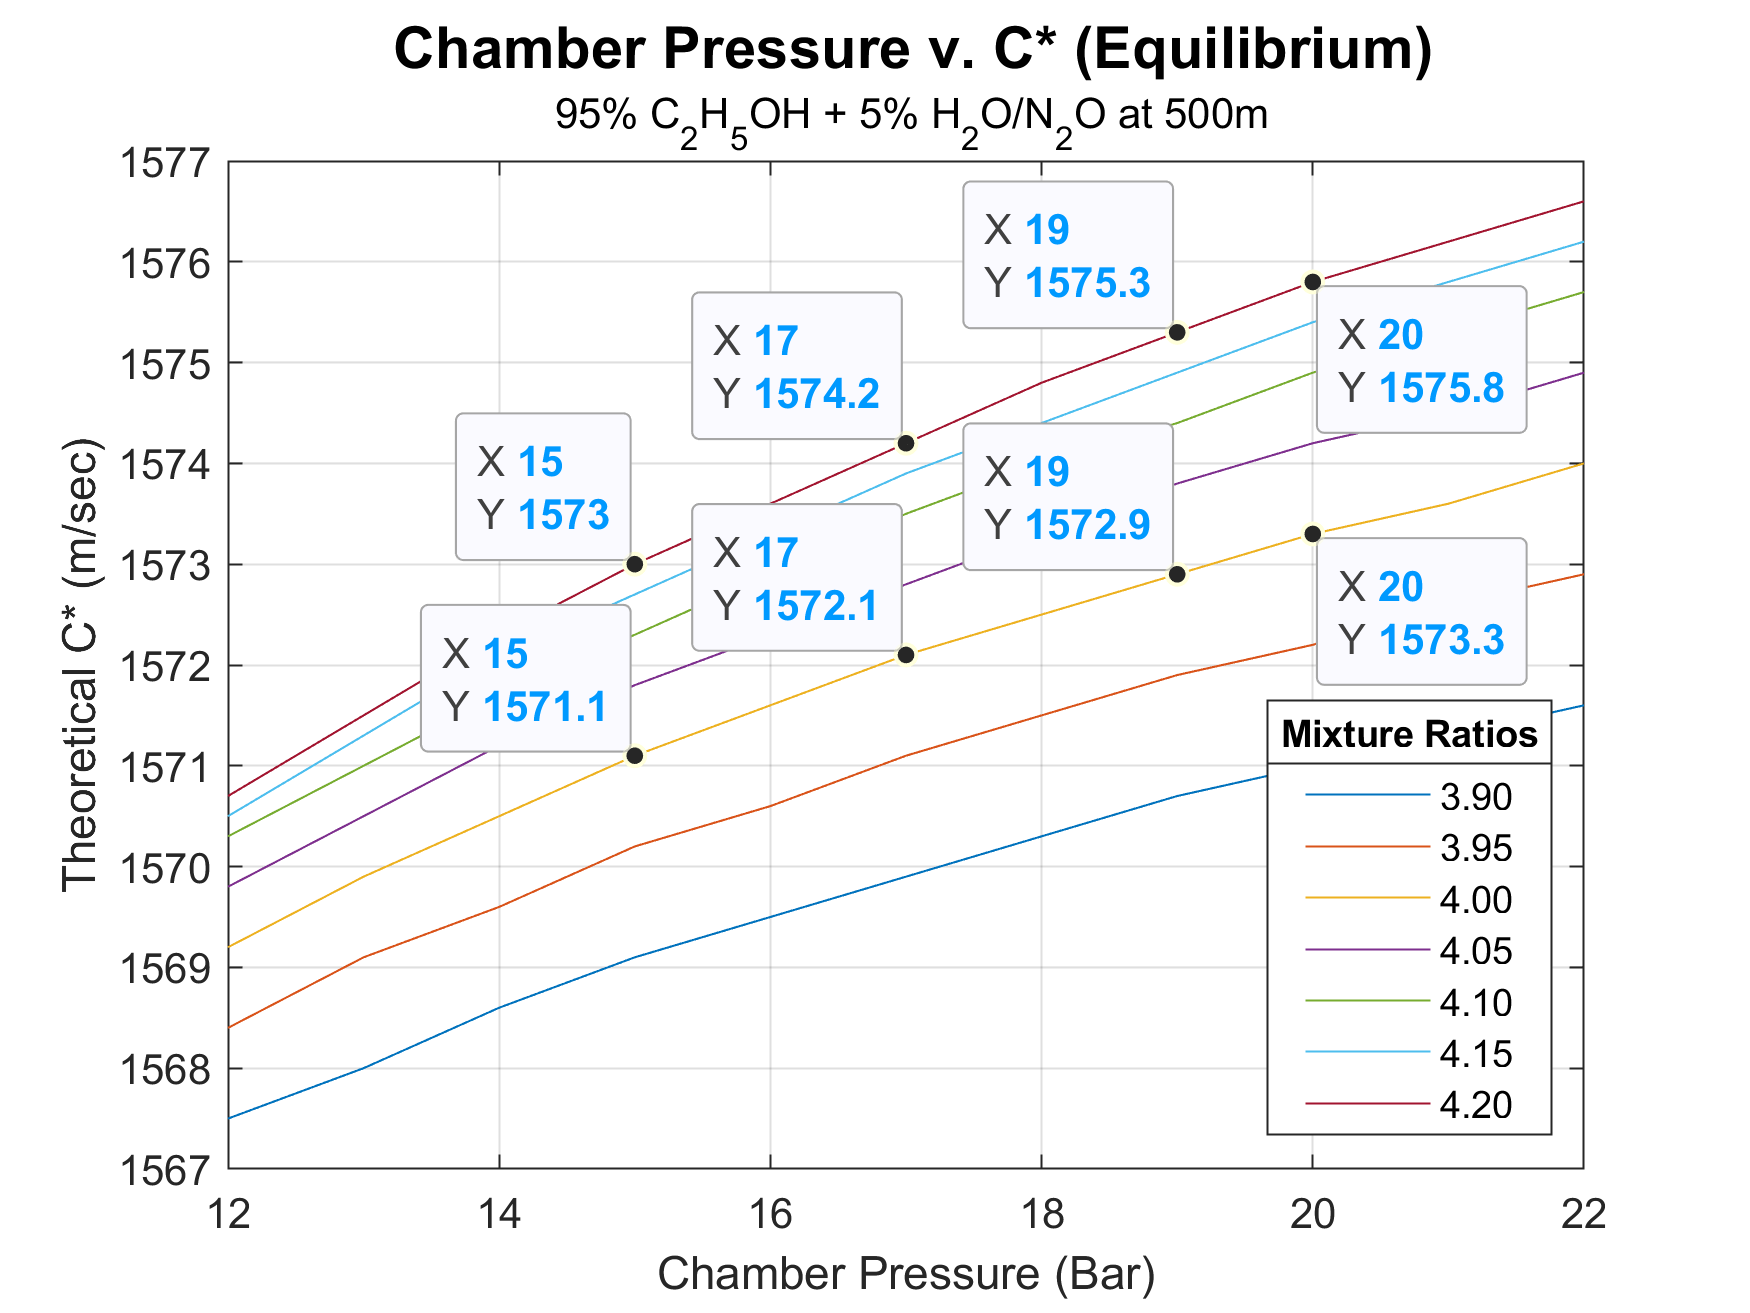
\includegraphics[scale=0.5, width=0.9\textwidth]{cp_cstar_mix_labeled} % first figure itself
        \caption{Theoretical C* efficiency vs chamber pressure and numerous mixture ratios.}
        \label{fig:cp_cstar}
    \end{minipage}\hfill
    \begin{minipage}{0.475\textwidth}
        \centering
        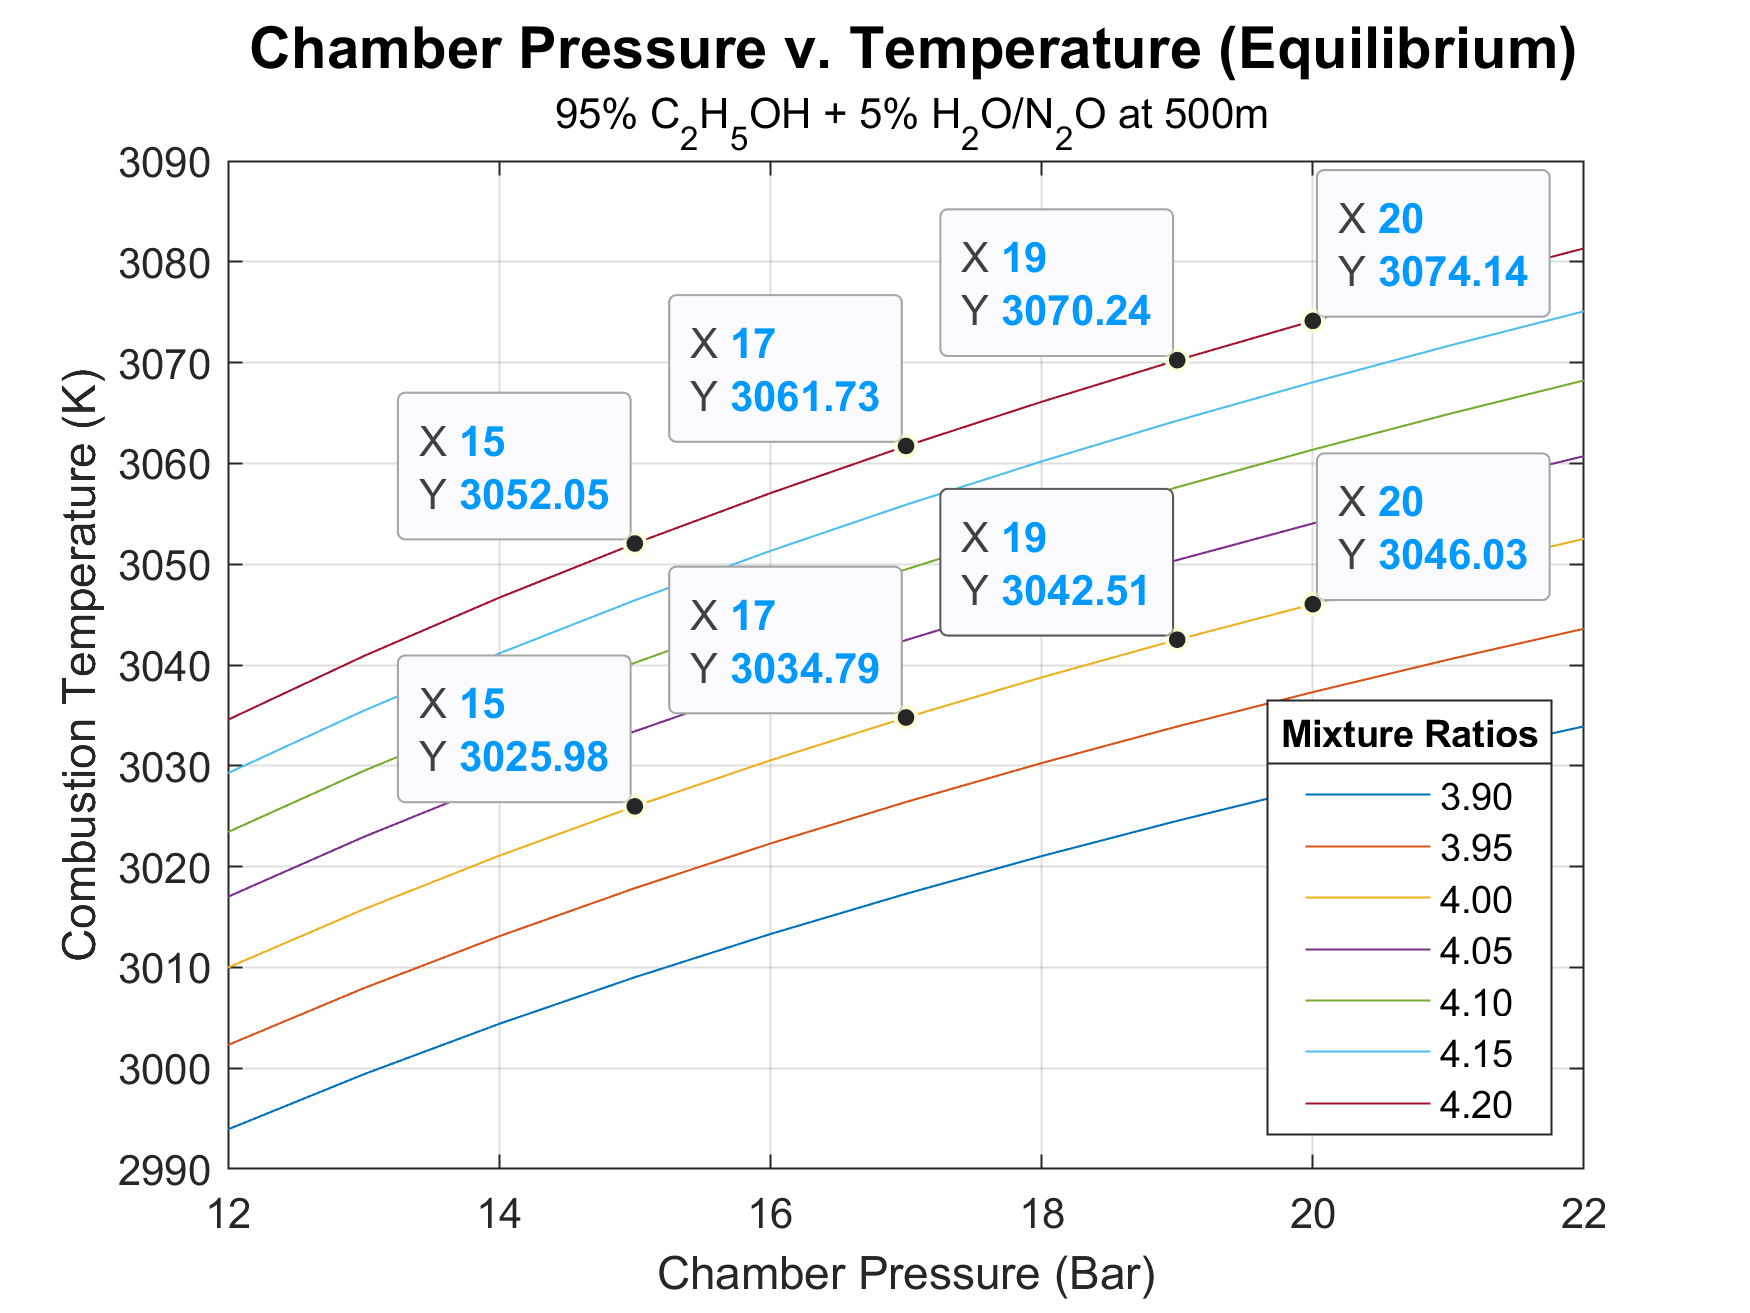
\includegraphics[scale=0.5, width=0.9\textwidth]{cp_temp_mix_labeled} % second figure itself
        \caption{Combustion temperature vs chamber pressure and numerous mixture ratios.}
        \label{fig:cp_temp}
    \end{minipage}
\end{figure} 
\begin{figure}
    \centering
    \begin{minipage}{0.475\textwidth}
        \centering
        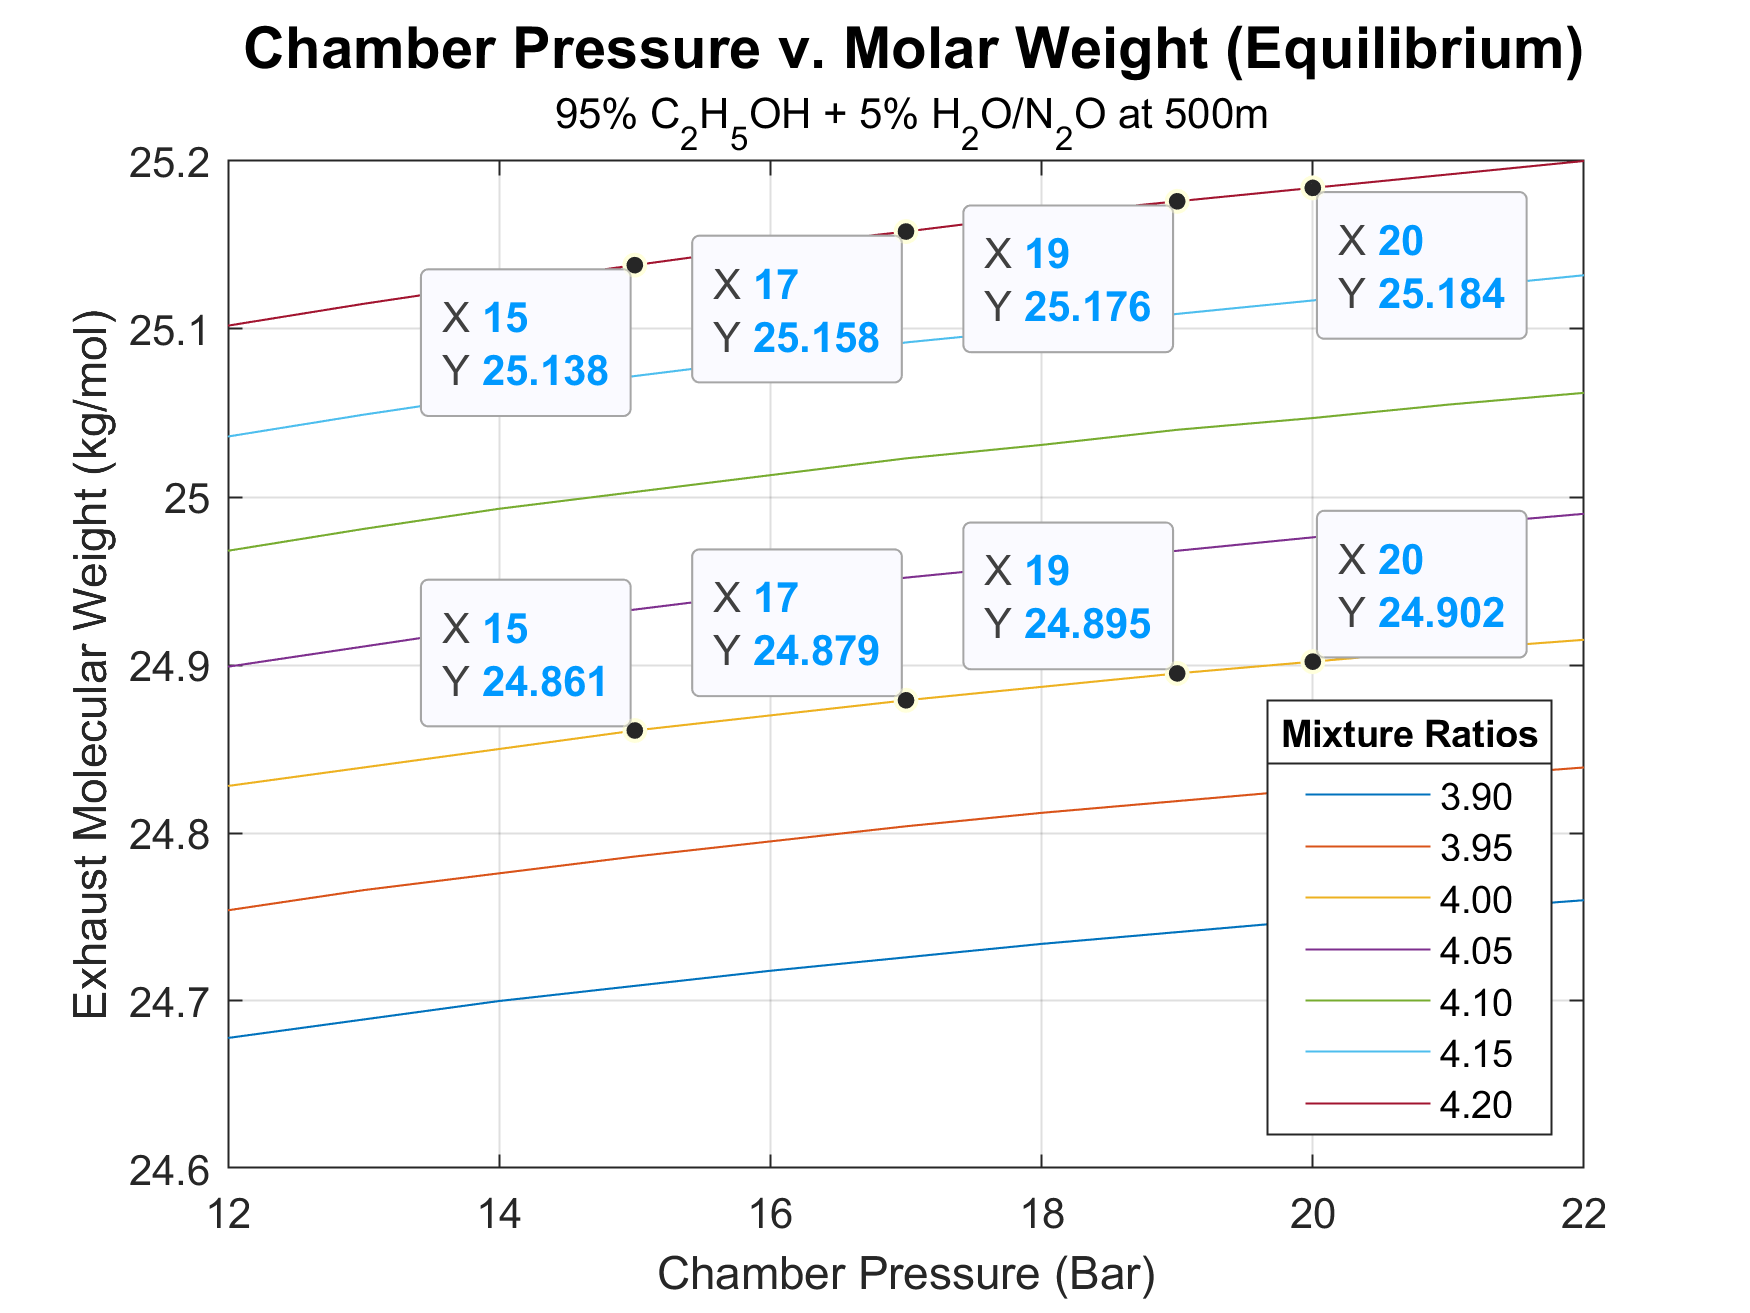
\includegraphics[scale=0.5, width=0.9\textwidth]{cp_molar_mix_labeled} % first figure itself
        \caption{Gas molecular mass vs chamber pressure and numerous mixture ratios.}
        \label{fig:cp_molar}
    \end{minipage}\hfill
    \begin{minipage}{0.475\textwidth}
        \centering
        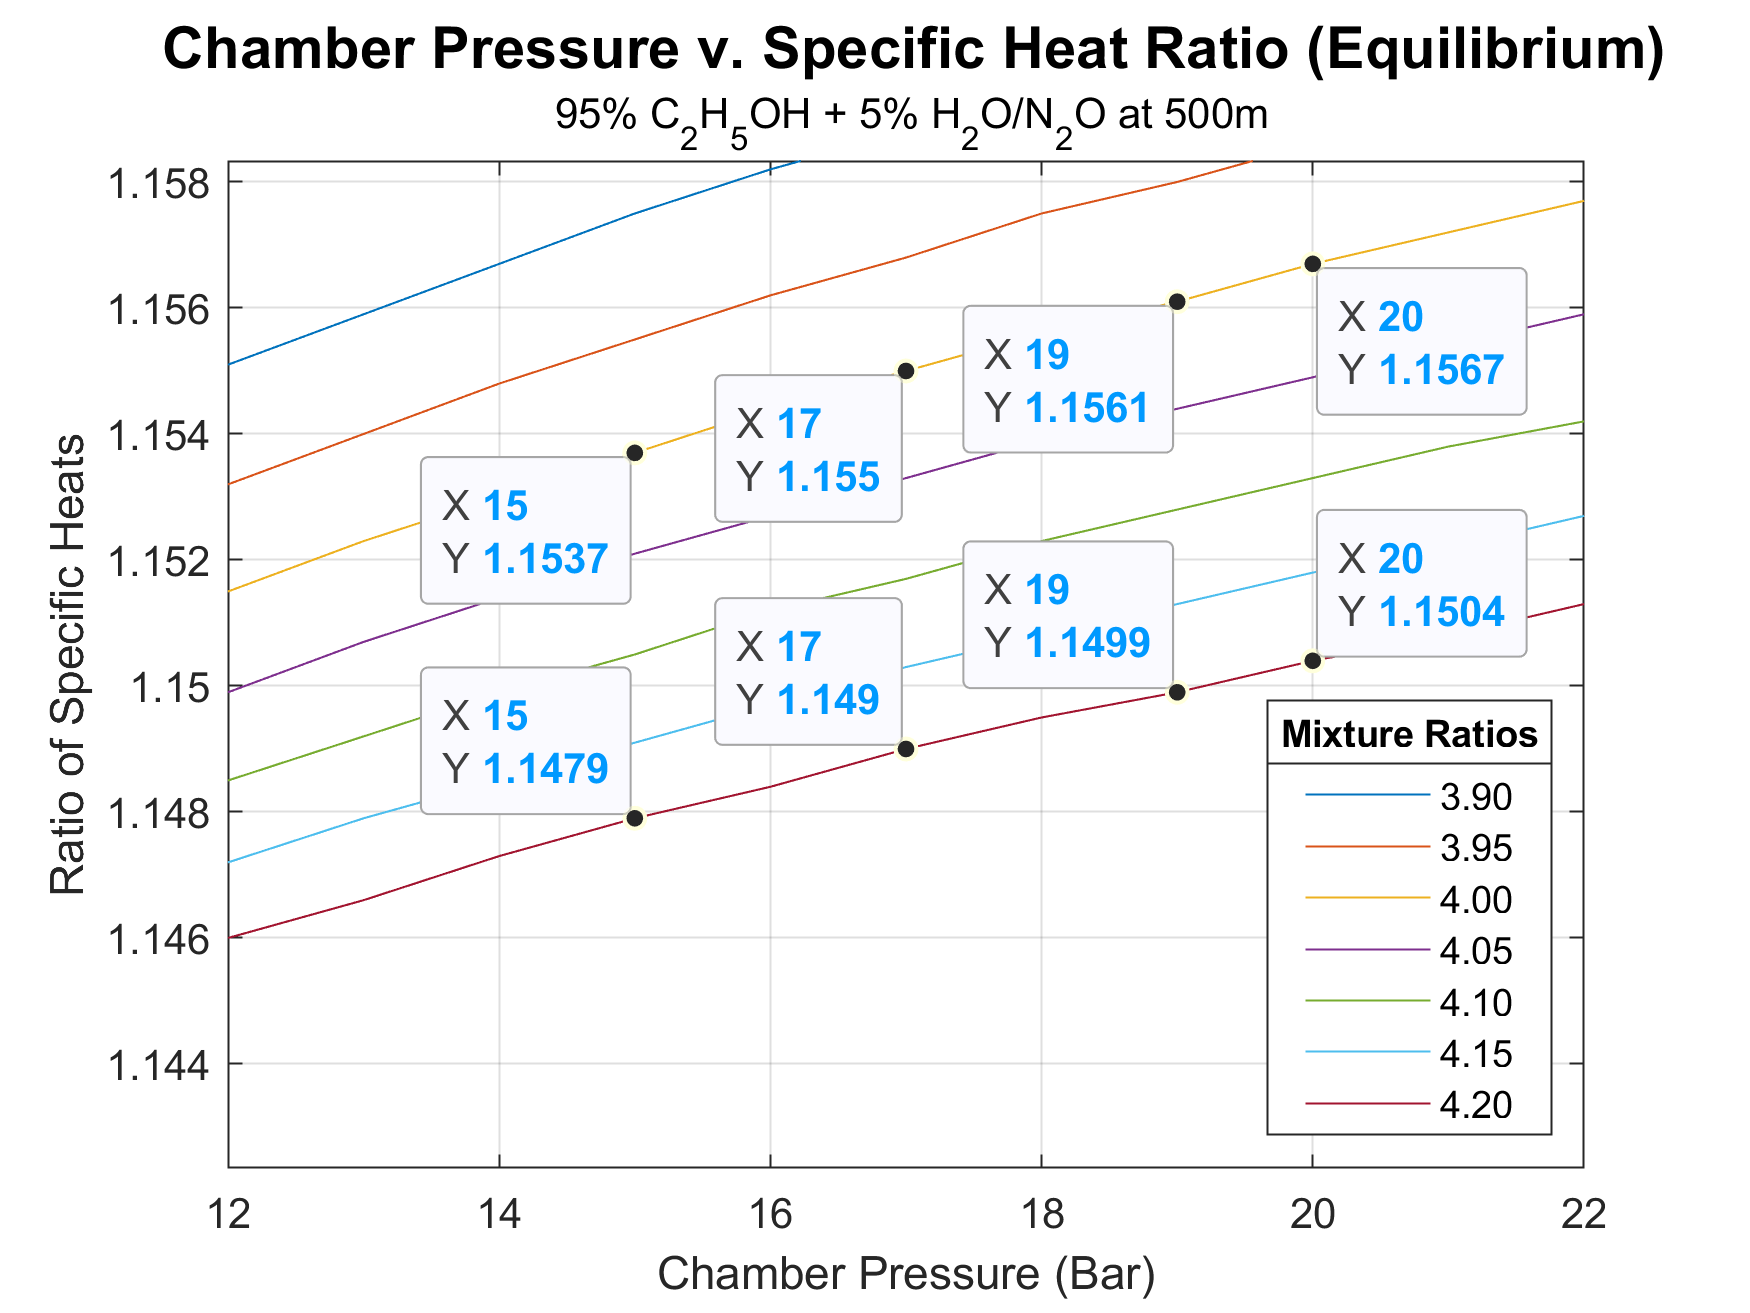
\includegraphics[scale=0.5, width=0.9\textwidth]{cp_gamma_mix_labeled} % second figure itself
        \caption{Ratio of specific heats vs chamber pressure and numerous mixture ratios.}
        \label{fig:cp_gamma}
    \end{minipage}
\end{figure}

\subsubsection{Chamber Pressure and Mixture Ratio Selection}
\hspace{\parindent} The first step is to realize the theoretical maximum performance to be expected from our propellant combination.  95\% ethyl alcohol (ethanol) was chosen for its availability, low pricing, and a modest specific impulse. A 95\% dilution (by mass) with water was chosen as to lower the expected combustion chamber temperature. This tradeoff sacrifices some $I_{sp}$ but reduces engineering complexity as regenerative and film cooling circuits may not be required. Industrial nitrous oxide was chosen as the main oxidizer for its self-pressurizing characteristics, non-cryogenic nature as opposed to liquid oxygen, relative ease to obtain, and a modest $I_{sp}$ with ethanol.
Using CEA, an open-source thermodynamics library provided by NASA's Glenn Research Center, critical data describing propellant combustion characteristics could be obtained. Numerical Python scripts were written to iterate through various combustion chamber pressures and mixture ratios and interface with CEA, and MATLAB scripts were used to parse and graph the CEA outputs as shown in Figures \ref{fig:cp_cstar}, \ref{fig:cp_temp}, \ref{fig:cp_molar}, and \ref{fig:cp_gamma}. Mixture ratios of 4.0 and 4.2 are labeled at certain chamber pressures. All dependent-variable properties (characteristic velocty $C^{*}$, combustion temperature $T_{c}$, exhaust molar mass $M$, and exhaust specific heat ratio $\gamma$) were permutated assuming shifting equilibrium flow and at an operational altitude of 500 m. 

A mixture ratio of 4.0 was chosen for Aphlex 1B mainly in the interest of a conservative combustion temerature of around 3026 K and a middle-of-the-line theoretical $C^{*}$ of around 1570 m/s, given a chamber pressure of 15 bar. This chamber pressure was chosen to minimize upstream fluid pressures and thus tank weight requirements, while also considering two additional design constraints that were not mentioned above but are nevertheless valid guiding parameters: a fluid flow velocity of less than 6 m/s to avoid water hammer effects [Zucrow Laboratories] and a pressure drop across the injector of around 25\% of the designated chamber pressure [Michigan Aeronautical Science Association]. The former of these additional guidlines is to avoid feed-coupled combustion instabilities that may be observed when the $\delta p$ across the injector is not adequately high. These guidelines further encourage a lower chamber pressure, and thus a conservative value of 15 Bar was chosen.

\subsubsection{Nozzle Design}

\begin{table}[!htb]
\centering
\begin{tabular}{ |p{5cm}||p{4cm}|p{1cm}|p{2cm}|  }
\hline
\multicolumn{4}{|c|}{Design Parameters} \\
\hline
Name & Value & Unit & Uncertainty \\
\hline
Propellant (Fuel)  &  Ethanol ($C_{2}H_{5}OH$, $95\%$)   &  N/A  &  N/A \\
Propellant (Oxidizer)  &  Nitrous oxide ($N_{2}O$) & N/A  &  N/A \\
$O/F$, Oxidizer/fuel ratio &  4.0  &  $N/A$  &   $\pm 1 \%$ \\
$F_{t}$, Nominal thrust &  1.50 &  $kN$  &  $\pm 0.1 \%$ \\
$P_{c}$, Chamber static pressure &  $1.5 \times 10^{6}$  &  $Pa$  &  $\pm 0.1 \%$ \\
$P_{e}$, Ambient pressure &  $9.5540 \times 10^{4}$  &  $Pa$  &  $\pm 0.1 \%$ \\
$T_{c}$, Chamber static temperature &  3025.98  &  $K$  &  $\pm 0.01 \%$  \\
$M$, Exhaust molecular mass &  24.861  &  $kg/mol$  &   $\pm 0.01 \%$ \\
$\gamma$, Specific heat ratio  &  1.1537  &  $N/A$  &   $\pm 0.001 \%$ \\
\hline
\end{tabular}
\caption{Summary of exhaust gas properties and fluid parameters.}
\label{table:gas_parameters}
\end{table}

\begin{equation} \label{eq:ambient_temperature}
T_{3} = 15.04 - 0.00649 h 
\end{equation}
\begin{equation} \label{eq:ambient_pressure}
P_{3} = \left[101.29 \times \left( \frac{T + 273.1}{288.08} \right) ^ {5.256} \right] \times 1000
\end{equation}

The nozzle design process followed standard procedures outlined in Rocket Propulsion Elements \cite{rpe} and open-source NASA documents. The thermodynamic properties of the exhaust gas and other important parameters are summarized and compiled in Table \ref{table:gas_parameters}. The ambient pressure was calculated using NASA Glenn Research Center's Earth Atmosphere Model for an altitude within the troposphere (less than 11000 meters), as shown in Equations \ref{eq:ambient_temperature} and \ref{eq:ambient_pressure}, where $T_{3}$ represents the ambient temperature in Kelvin, $h$ is the altitude in meters, $P_{3}$ is the ambient pressure in Pascals.

Assuming fully isentropic flow (by definition both adiabatic and reversible) in the supersonic nozzle with choked flow conditions at the throat, an ideal converging-diverging (de Laval) nozzle can be characterized. The first parameter to calculate is the controlling area ratio
\begin{equation} \label{eq:area_ratio}
\frac{A_{t}}{A_{2}} = \left( \frac{\gamma + 1}{2} \right) ^{1/(\gamma - 1)} \left( \frac{p_{2}}{p_{1}} \right) ^{1/\gamma} \sqrt{ \frac{\gamma + 1}{\gamma - 1} \left[ 1 - \left( \frac{p_{2}}{p_{1}} \right) ^{(\gamma - 1)/\gamma} \right] }
\end{equation}
where $A_{t}$ is the cross-sectional area of the throat, $A_{2}$ is the cross-sectional area at nozzle exit, and $p_{1}$ and $p_{2}$ are the chamber pressure and exit pressure respectively. Equation \ref{eq:area_ratio} is also often referred to as the inverse of the expansion ratio $\epsilon$, since $\epsilon = A_{2}/A_{t}$. Evaluating Equation \ref{eq:area_ratio} gives
\begin{equation*} 
\frac{A_{t}}{A_{2}} = \left( \frac{2.15}{2} \right) ^{1/0.15} \left( \frac{9.6 \times 10^{4}}{1.5 \times 10^{6}} \right) ^{1/1.15} \sqrt{ \frac{2.15}{0.15} \left[ 1 - \left( \frac{9.6 \times 10^{4}}{1.5 \times 10^{6}} \right) ^{0.15/1.15} \right] } = 0.307
\end{equation*}
Notice the substitution of $p_{2}$ for $P_{e}$ as specified in Table \ref{table:gas_parameters}, since in an ideal nozzle, the exhaust gas should expand to ambient pressure. The expansion ratio $\epsilon$ is simply
\begin{equation*}
\epsilon = A_{2}/A_{t} = 1/AR = 1/0.307 = 3.26
\end{equation*}
Next, we can find the ideal exit velocity $v_{2}$, sometimes denoted as $c$:
\begin{equation} \label{eq:exit_velocity}
v_{2} = \sqrt{ \frac{2\gamma}{\gamma - 1} \left( \frac{R_{u}T_{1}}{M} \right) \left[ 1- \left( \frac{p_{2}}{p_{1}} \right) ^{(\gamma - 1)/\gamma} \right] }
\end{equation}
where $R_{u}$ is the universal gas constant of 8314.3 J/kg mol-K and $M$ is the molecular mass of the gas as shown in Table \ref{table:gas_parameters}. Evaluating gives
\begin{equation*} 
v_{2} = \sqrt{ \frac{2 * 1.15}{0.15} \left( \frac{8314.3 * 3026}{24.86} \right) \left[ 1- \left( \frac{9.6 \times 10^{4}}{1.5 \times 10^{6}} \right) ^{0.15/1.15} \right] } = 2162.3 \; m/s
\end{equation*}
Next, the mass flow rate $\dot{m}$ can be calculated explicitly noting that $v_{2} = c$, since earlier it was stated that $p_{2} = p_{3}$:
\begin{equation} \label{eq:mdot}
\dot{m} = F_{t}/c = 1500/2162.3 = 0.694 \; kg/s
\end{equation}
Solving using our chosen $O/F$ ratio of 4.0 for each independent propellant $\dot{m}$ gives
\begin{align*} 
\dot{m}_{o} = \dot{m} * (4/5) = 0.694 * (4/5) = 0.555 \; kg/s \\
\dot{m}_{f} = \dot{m} * (1/5) = 0.694 * (1/5) = 0.139 \; kg/s
\end{align*}
Next, we arrive at the throat area:
\begin{equation} \label{eq:throat_area}
A_{t} = \frac{\dot{m}}{p_{1}} \sqrt{ \frac{(R_{u}/M)T_{1}}{\gamma [2/(\gamma + 1)]^{(\gamma + 1)/(\gamma - 1)}} }
\end{equation}
Evaluating Equation \ref{eq:throat_area} gives
\begin{equation*} 
A_{t} = \frac{0.694}{1.5 \times 10^{6}} \sqrt{ \frac{(8314.3/24.86) * 3026}{1.15 [2/(2.15)]^{(2.15)/(0.15)}} } = 7.29 \times 10^{-4} \; m^{2} = 7.29 \; cm^{2}
\end{equation*}
Using this calculated throat area and the expansion ratio, the exit area is simply
\begin{equation} \label{eq:exit_area}
A_{2} = \epsilon * A_{t} = 3.26 * 7.29 \times 10 ^{-4} = 2.38 \times 10^{-3} \; m^{2} = 23.8 \; cm^{2}
\end{equation}
From the parameters calculated thus far, we can calculate some useful performance metrics such as $I_{sp}$ and thrust coefficient $C_{F}$:
\begin{equation} \label{eq:specific_impulse}
(I_{sp})_{opt} = F_{t}/(\dot{m} * g_{0}) = c/g_{0} = 2162.3/9.81 = 220.42 \; sec
\end{equation}
where $g_{0}$ is the acceleration due to gravity at Earth's surface. $C_{F}$ is
\begin{equation} \label{eq:thrust_coefficient}
(C_{F})_{opt} = \frac{F_{t}}{p_{1}A_{t}} = \frac{1500}{1.5 \times 10^{6} * 7.29 \times 10 ^{4}} = 1.372
\end{equation}
Note that under a more rigorous derivation, $C_{F}$ can be seen to be a key parameter for analysis and varies depending on $\gamma$, the nozzle expansion ratio $\epsilon$, and the pressure ratio $p_{1}/p_{2}$. Normally, $C_{F}$ is experimentally determined by measuring chamber pressure, throat diameter, and thrust. The optimal $C_{F}$ and therefore $F_{t}$ occur when $p_{2} = p_{3}$.

Finally, the physical dimensions of the nozzle can be determined using simple trigonometry via a standard convergence half-angle $\alpha$ of $\ang{45}$ and a standard divergence half-angle $\beta$ of $\ang{15}$. The characteristic chamber length $L^{*}$, a parameter used for characterizing the necessary chamber volume for adequate mixing and combustion of the propellants, must be more carefully considered. Ideally, $L^{*}$ is purely a function of the chemistry of the propellant combination and is often based upon previous successful engine designs \cite{rpe}. However, due to the dynamical and complex nature of nitrous oxide, such as exothermic decomposition after vaporization in the injector and a high density sensitivity to temperature, a more sophisticated model is needed to calculate $L^{*}$. Palacz proposes an explicit equation for finding the ideal $L^{*}$ for a nitrous oxide system, and empirically determined an ideal range for an $NO_{x}$/ethanol system of $L^{*}$ values from 125.6 cm to 167.8 cm \cite{nitrous-paper}. This range is confirmed by Sutton and Biblarz, as $L^{*}$ values of between 1.0 m and 1.5 m are expected with ethanol systems. A low-range $L^{*}$ value of 1.25 m was chosen as a smaller form factor is desired over perfect combustion efficiency. $L^{*}$ is mathematically defined as simply
\begin{equation} \label{eq:l_star}
L^{*} = \frac{V_{c}}{A_{t}} = \frac{\pi r_{c}^{2} L{c}}{A_{t}} \; \Longrightarrow \; L_{c} = \frac{A_{t} L^{*}}{\pi r_{c}^{2}}
\end{equation}
where $L_{c}$ is the length of the chamber and $r_{c}$ is the radius of the chamber. It is apparent that the a desired form factor can be obtained by adjusting either the radius or the length of the chamber. Through iteration, a chamber radius $r_{c}$ of 4.0 cm was chosen. The only constraint on the chamber radius is the contraction ratio, defined as $A_{1}/A_{t}$ (the ratio of chamber area to throat area), which must achieve a value of 4.0 or more \cite{rpe}. A trivial area calculation can be performed to confirm that this constaint is satisfied: $CR =  \pi r_{c}^{2}/A_{t} = 5.03 \times 10^{-4} \; m^{2} / 7.29 \times 10^{-4} \; m^{2} = 6.90 > 4.0$. The chamber length is therefore
\begin{equation*}
L_{c} = \frac{A_{t} L^{*}}{\pi r_{c}^{2}} = \frac{(7.29 \times 10^{-4} \; m^{2})(1.25 \; m)}{5.03 \times 10^{-4} \; m^{2}} = 0.1813 \; m = 18.13 \; cm
\end{equation*}

\begin{table}[!htb]
\centering
\begin{tabular}{ |p{6cm}||p{2cm}|p{1cm}| }
\hline
\multicolumn{3}{|c|}{Calculated Performance Parameters} \\
\hline
Name & Value & Unit \\ 
\hline
$\dot{m}$, Total mass flow rate  &  0.694  &  $kg/s$  \\
$\dot{m}_{f}$, Fuel mass flow rate &  0.555  &  $kg/s$  \\
$\dot{m}_{o}$, Oxidizer mass flow rate &  0.139  &  $kg/s$  \\
$v_{2}$, Exhaust velocity & 2162.3 & $m/s$ \\
$(I_{sp})_{opt}$, Specific impusle (optimal) & 220.42 & $s$ \\
$(C_{F})_{opt}$, Thrust coefficient (optimal) & 1.372 & $N/A$ \\
\hline
\end{tabular}
\caption{Summary of engine performace parameters.}
\label{table:calculated_parameters}
\end{table}

\begin{table}[!htb]
\centering
\begin{tabular}{ |p{6cm}||p{2cm}|p{1cm}| }
\hline
\multicolumn{3}{|c|}{Calculated Dimensional Parameters} \\
\hline
Name & Value & Unit \\ 
\hline
$\alpha$, Convergence half-angle &  45  &  $deg$ \\
$\beta$, Divergence half-angle &  15  &  $deg$  \\
$A_{t}$, Throat area  & $7.29 \times 10^{-4}$ & $m^{2}$ \\
$A_{2}$, Exit area & $2.38 \times 10^{-3}$ & $m^{2}$ \\
$A_{c}$, Chamber cross-sectional area & $5.03 \times 10^{-4}$ & $m^{2}$ \\
$R_{t}$, Throat radius & $15.23$ & $mm$ \\
$R_{2}$, Exit radius & $27.52$ & $mm$ \\
$R_{c}$, Chamber radius & $40.0$ & $mm$ \\
$L_{c}$, Chamber length & $181.3$ & $mm$ \\
$\epsilon$, Expansion ratio  &  3.26  &  $N/A$  \\
$CR$, Contraction ratio  &  6.9  &  $N/A$  \\
\hline
\end{tabular}
\caption{Summary of physical nozzle dimensions.}
\label{table:calculated_dimensions}
\end{table}

Table \ref{table:calculated_parameters} shows the engine parameters calculated so far in this section, while Table \ref{table:calculated_dimensions} shows the physical nozzle dimensions calculated so far in this section. Using the data from Table \ref{table:calculated_dimensions}, a basic conical nozzle can be realized.

\begin{figure}
\centering
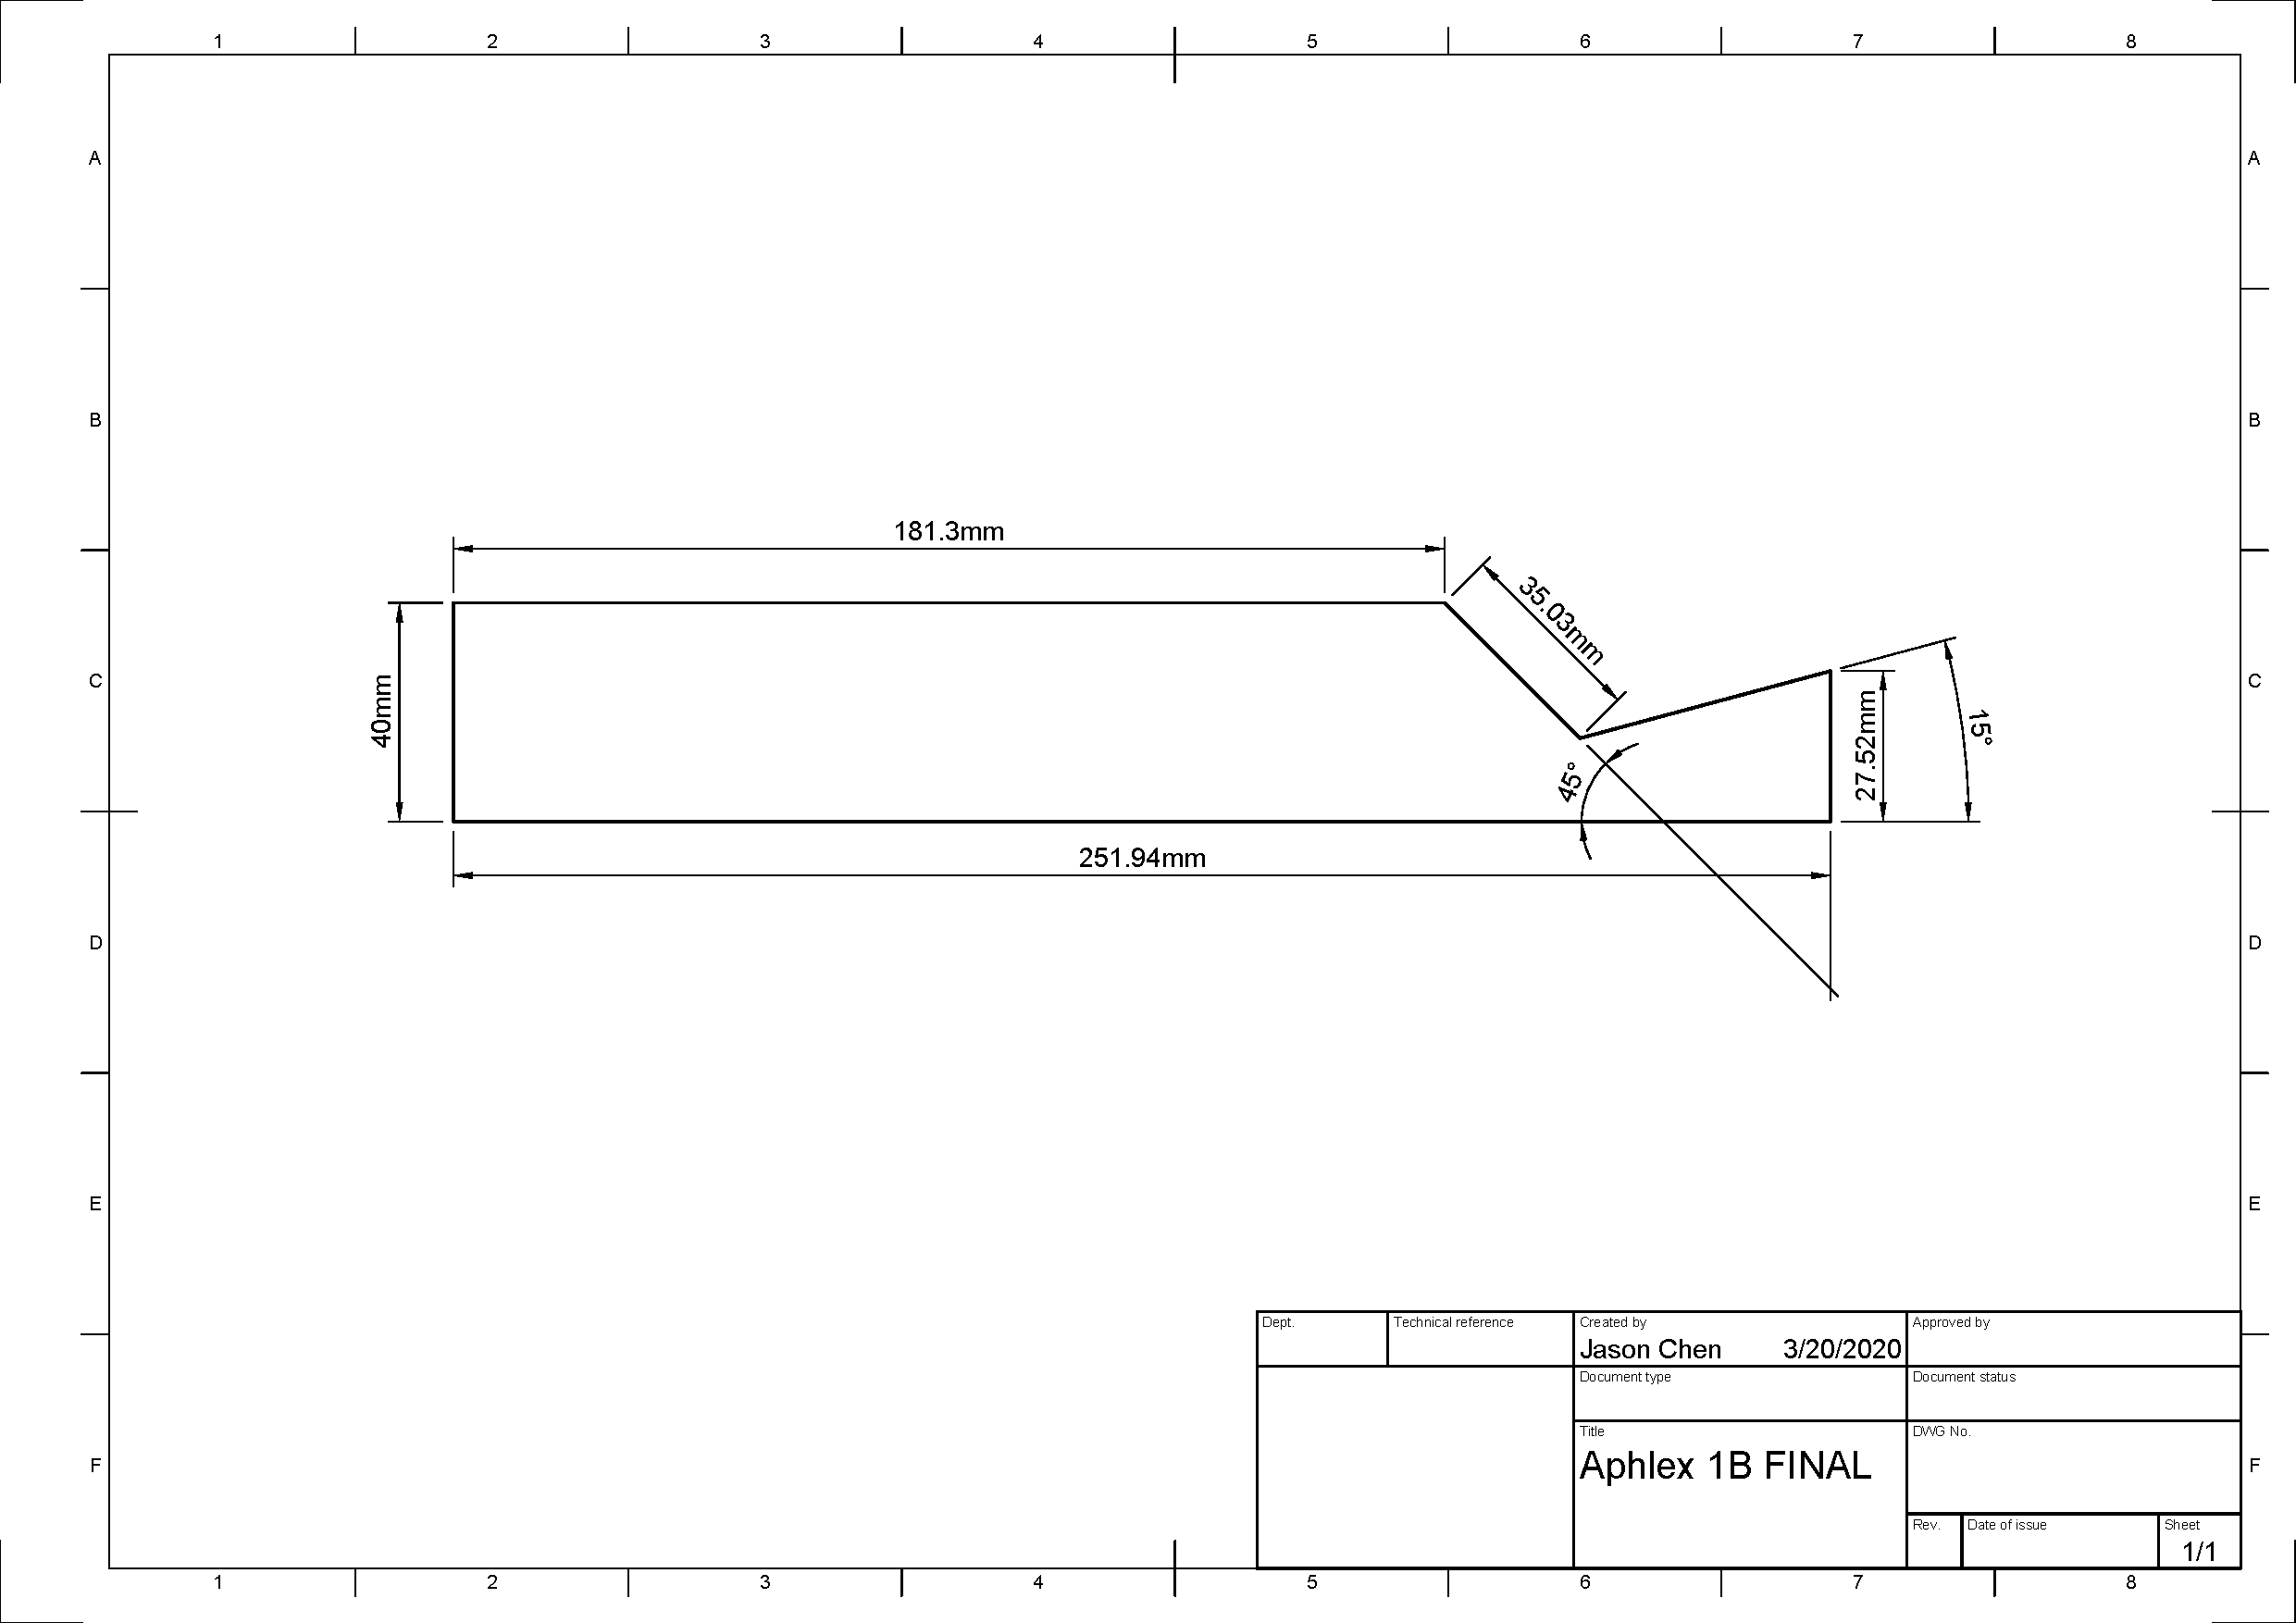
\includegraphics[scale=0.5, width=0.9\textwidth, trim={6.5cm 12.5cm 5.5cm 9cm}, clip]{aphlex1b-drawing} % Trim order is left, bottom, right, top
\caption{Aphlex 1B drawing with a conical nozzle and given dimensions.}
\label{fig:conical_nozzle_drawing}
\end{figure}

[Add section on finding $I_{sp}$ and $F_{t}$ at launch and MECO, along with a table of physical nozzle design parameters and their calculated dimensions.]

\subsection{Callisto 1}

\subsection{Injector Design}

\hspace{\parindent} The injector types considered were the triplet (fuel-centered) unlike impinging injector and the like-on-like doublet impinging injector, due to 1) our limited manufacturing capabilities 2) a fairly unbalanced O/F ratio 3) both types exhibiting good mixing and atomization properties and 4) the abundance of historical experience and data with both injector types. NASA's SP-8089 conference document on liquid engine injector design suggests that the best way to characterize both the individual orifice geometries and the overall injector geometry for unlike impinging injectors is through diameter ratios. Vigorous cold flow and other empirically testing methods at the time were used and have found correlations between the driving orifice diameter ratio with the optimum mixing efficiency. The correlation found was
\begin{equation} \label{eq: diameter_ratio}
    \left( \frac{d_{c}}{d_{ou}} \right)^{2} = M \left[ \frac{\rho_{ou}}{\rho_{c}} \left( \frac{\dot{m}_{c}}{\dot{m}_{ou}} \right)^{2} \right]^{0.7}
\end{equation}
where $d_{c}$ is the diameter of center orifice, $d_{ou}$ is the diameter of an outside individual orifice, M is an experimentally-determined mixing factor coefficient, $\rho$ represents liquid density, and $\dot{c}$ and $\dot{m}_{ou}$ are the center mass flow rate and outside mass flow rate respectively. It is cited that for a 2-on-1 element type, M has a value of 1.6. Using Equation \ref{eq: diameter_ratio}, we find that our controlling diameter ratio is
\begin{equation*}
    \frac{d_{c}}{d_{ou}} = \sqrt{M \left[ \frac{\rho_{ou}}{\rho_{c}} \left( \frac{\dot{m}_{c}}{\dot{m}_{ou}} \right)^{2} \right]^{0.7}} = \sqrt{1.6 \left[ \frac{772.25 \; kg/m^{3}}{789 \; kg/m^{3}} \left( \frac{0.1389 \; kg/s}{0.5556 \; kg/s} \right)^{2} \right]^{0.7}} = 0.4757
\end{equation*}
Since this diameter ratio is not reasonably near 1.22 (as suggested by NASA SP-8089), we can assume this correlation would not be accurate and that there will be potentially drastic losses in mixing efficiency. Thus, this suggests that a like-on-like system is required. Since like-on-like elements will have a 1 to 1 diameter and momentum ratio, we can begin determining the pressure drop and mass flow rate through each individual orifice. Rocket Propulsion Elements (RPE) provides and equation for the volumetric flow rate $Q$ (and therefore $\dot{m}$ since $\rho$ is constant) as shown below:
\begin{equation} \label{eq: discharge}
    \dot{m} = Q \rho = C_{d} A \sqrt{2 \rho \Delta p} \; \Longrightarrow \;
    \Delta p = \left[ \left( \frac{\dot{m}}{C_{d} A} \right)^{2} \right] / 2 \rho
\end{equation}
where $C_{d}$ is a dimensionless discharge coefficient that is experimentally determined and a function of the orifice geometry, $A$ is the area of the orifice, and $\Delta p$ is the pressure drop across the orifice. Flow velocity is similar:
\begin{equation} \label{eq: flow_velocity}
    v = Q/A = C_{d} \sqrt{2 \Delta p /\rho}
\end{equation}
Since $C_{d}$ is a measured parameter, initial design calculations must assume a value. RPE suggests a $C_{d}$ value of around 0.88 for a 1 mm diameter orifice in a short tube with a rounded entrance (L/D $>$ 3.0), and 0.9 for a similar configuration with a 1.57 mm diameter. Accordingly, a $C_{d}$ value of 0.9 was chosen for the oxidizer and a $C_{d}$ value of 0.88 was chosen for the fuel. For the orifice sizing, NASA SP-8089 found that smaller orifice sizes attributed to better mixing in all scenarios, although only to a certain extent (orifice diameters $<$0.03 inches saw insignificant improvements in mixing). Due to limited manufacturing capabilities, a minimum hole size of 1 mm was chosen. Using this information, a design parameter of an overall injector pressure drop that is 25$\%$ of chamber pressure, and Equation \ref{eq: discharge}, the mass flow rate across a single oxidizer and fuel orifice are
\begin{equation*}
    \dot{m}_{o} = 0.9*(\pi*((1.58 \; mm/2)\times 10^{-3})^{2}) \sqrt{2(772.25 kg/m^{3})(1.5 \times 10^{6} \; Pa * 0.25)} = 0.0425 \; kg/s
\end{equation*}
\begin{equation*}
    \dot{m}_{f} = 0.88*(\pi*((1.00 \; mm/2)\times 10^{-3})^{2}) \sqrt{2(789 kg/m^{3})(1.5 \times 10^{6} \; Pa * 0.25)} = 0.0168 \; kg/s
\end{equation*}
The same pressure drops can be used for each orifice due to Bernoulli's principle and the law of conservation of energy, similar to how voltage stays constant across a parallel circuit. The corresponding injection velocities (Equation \ref{eq: flow_velocity}) are
\begin{equation*}
    v_{o} = 0.9 \sqrt{(2(1.5\times 10^{6} \; Pa)(0.25))/(772.25 \; kg/m^{3})} = 28.048 \; m/s
\end{equation*}
\begin{equation*}
    v_{f} = 0.88 \sqrt{(2(1.5\times 10^{6} \; Pa)(0.25))/(789 \; kg/m^{3})} = 27.132 \; m/s
\end{equation*}
Dividing the mass flow rate by the individual orifice mass flow rates gives the total orifice count for each propellant:
\begin{equation*}
    Number \; of \; oxidizer \; orifices = \dot{m}_{o}/\dot{m}_{oi} = (0.4865 \; kg/s)/(0.0425 \; kg/s) = 11.447
\end{equation*}
\begin{equation*}
    Number \; of \; fuel \; orifices = \dot{m}_{f}/\dot{m}_{fi} = (0.139 \; kg/s)/(0.0168 \; kg/s) = 8.27
\end{equation*}
Since an integer and even amount of holes are required for a like-on-like impinging injector, Equation \ref{eq: discharge} is rearranged to compute the necessary diameter given the desired number of orifices, given a reasonable range of orifice count provided by the previous calculation:

Thus, to achieve [x] oxidizer orifices and [y] fuel orifices

an oxidizer orifice diameter of [x] mm and fuel orifice diameter of [y] mm are needed.
Remaining impingement injector parameters were chosen due to a literature review, rather than explicit calculations. The angle of impingement, $\lambda$, is chosen to be 60 degrees (relative to the injector axis) and a point of impingement of around 3 cm downstream of the injector face is chosen for maximum ethanol/nitrous oxide combustion efficiency. The final injector parameters are summarized in the table below.
[Still need to figure out angle of impingement, distance from injector face, though this is expected to be 60 degrees and around 3 cm respectively. Need to note that L/D is greater than 3 (or more), and that higher is better.]

\subsection{Plumbing System}
The following section describes the theoretical process used to dimensionalize the prelimiary plumbing framework in preparation for the first static cold flow test. By definition, these calculations are purely speculatory and are only used for the initial design process. The purpose of the cold flow test is to verify these parameters, and consequently adjust these parameters to better fit the system requirements.
\subsubsection{Assumptions} \label{sec:assumptions}

To simplify the rigorous analysis and optimization processes often associated with viscous pipe flow, a couple of assumptions are applied in the following section to both shorten the development timeline and to avoid unecessarily complex or expensive methods outside of the scope of a high school amateur rocketry program. They are as follows:
\begin{enumerate}
\item Flow is driven by both pressure and gravity.
\item Pipe is circular and is of constant cross-sectional area. \label{itm:constant-area}
\item No swirl, circumferential variation, or entrance effects.
\item No shaft-work or heat-transfer effects. \label{itm:heat-effects}
%\item A simplified steady-flow energy equation due to Assumption \ref{itm:heat-effects}.
\item Flow is fully developed (minimal boundary-layer effects).
\end{enumerate}

\begin{table}[!htb]
\centering
\begin{tabular}{ |p{4cm}||p{4cm}|p{2cm}|p{2cm}|  }
\hline
\multicolumn{4}{|c|}{Design Parameters} \\
\hline
Name & Value & Unit & Uncertainty \\
\hline
$\mu$, Dynamic viscosity  &  0.00196  &  $kg/m \cdot s$  &  $\pm 0.1 \%$ \\
$\rho$, Density  &  786  &  $kg/m^{3}$  &  $\pm 1 \%$ \\
$L$, Pipe length  &  8.0  &  $m$  &  $\pm 0.1 \%$  \\
$d$, Pipe diameter  &  12.7  &  $mm$  &   $\pm 0.1 \%$ \\
$\dot{m}$, Mass flow rate  &  0.9133  &  $kg/s$  &   $\pm 0.1 \%$ \\
Pipe material  &  Hard nylon  &  N/A  &  N/A \\
$\epsilon$, Roughness  &  1.5 to 40.0  &  $\mu m$  &  $\pm 50 \%$ \\
\hline
\end{tabular}
\caption{Summary of exhaust gas properties and fluid parameters.}
\label{table:pipe_parameters}
\end{table}

\printbibliography
%\end{multicols}

\end{document}
